\documentclass[a4paper]{article}

\usepackage[utf8]{inputenc}
\usepackage[T1]{fontenc}
\usepackage{lmodern}
\usepackage[frenchb]{babel}

\usepackage{graphicx}
\usepackage{wrapfig}

\usepackage{amsmath}
\usepackage{amssymb}
\usepackage{chemfig}
\usepackage{cancel}

\usepackage{lettrine}
\usepackage{oldgerm}
\makeatletter
\@addtoreset{section}{part}
\makeatother

\begin{document}
\begin{center}
{\Huge \textbf{Projet TER RobotTaf}}
\\~
\\~
\\~
\\~
{\Large \textbf{Par:}}\\
\large{\textbf{Victor Coutellier - Julien Gauttier - Vladimir Karassouloff}}
\\~
\\~
\\~
\large{\textbf{Faculté des sciences d’Orléans -  M1 informatique}}
\\~
\\~
\\~
\end{center}

\tableofcontents
\newpage

\lettrine{L}'objectif de ce projet est de concevoir un mini langage servant à manipuler un robot afin d’enseigner les bases de la programmation aux jeunes enfants.
\\
Il s’agira de concevoir un langage de programmation contenant la plupart des notions de l’algorithmique et de le rendre accessible à des enfants. Une application Android devra être développer, les enfants devront alors créer un algorithme avec le langage préalablement conçu via cette application. Cette application servira d’interface entre l’enfant et le robot. Le programme produit par l’enfant devra ensuite être envoyé sur un robot qui lancera localement son exécution.

\section{Une introduction au domaine}

A l’origine, si l’apparition de la programmation à déclenché un élan d’apprentissage aux jeunes enfant, les premiers langages n’étais pas adaptées a ces derniers. En effet, la syntaxe était très exigeante et austère. De plus, la programmation était souvent introduite dans des contextes non familiers aux jeunes enfants, tel que la génération de nombres premiers, ou dessiner des formes géométriques.

\paragraph{}
Dans son livre \cite{Papert:1980:MCC:1095592}, Seymour Papert’s indique d’un language de programmation éducatif doit répondre à 3 critères
\begin{itemize}
\item « low-floor », c’est à dire simple d’accès
\item « high ceiling », c’est à dire fourni des opportunités de créer des projets complexe avec le temps
\item « wide-walls », c’est à dire suffisamment vaste pour engager different types de projets
\end{itemize}
Mais ces 3 contraintes n’étais pas satisfiables au vu des limitations techniques de l’époque.

\paragraph{}
Il est également remarqué d’une personne apprends mieux en travaillant sur des projets personnel, c’est pourquoi il est important d’insister sur
\begin{itemize}
\item La diversité des projets ( jeux, histoire, animations, simulations ), afin que chacun puisse se retrouver dans le langage utilisé
\item La personnalisation, il est donc important de pouvoir importer ses propres images, son, voix, ainsi que des outils pour créer ses propres ressources.
\item le choix de la 2D dans le développement d’une application d’apprentissage est donc plus approprié, car en effet, il est plus simple d’importer des assets 2D, tout comme il est plus simple de les personnaliser et de créer un environnement cohérents autour
\end{itemize}

\paragraph{}
Il fut également remarqué dans plusieurs études - notamment le département des sciences et de la technologie de l’éducation de l’université de Mons \cite{temperman:halshs-01092656}, et le Department of Psychologie of Nazarene College \cite{degelman1986concept} - que les enfants ayant été confrontés à des problèmes algorithmiques de façon ludique progresse de façon significative dans des problèmes mathématiques. Mais malgré cela, il fut aussi démontré que laisser l’enfant livré à lui-même dans un environnement de programmation ne suffit pas à developper ses capacités, le rôle de l’enseignant est primordial pour observer de réel effets positifs sur le développement de ces compétences.

\paragraph{}
« Si nous observons des gains d’apprentissage élevés dans le domaine des grandeurs, des nombres et de la structuration spatiale, l'impact du dispositif semble plus réduit pour les compétences relatives à la résolution de problèmes et pour le raisonnement logique. Un autre résultat intéressant qui ressort de notre analyse est l'effet du scénario en termes d’équité. Les résultats des apprenants sont en effet plus homogènes au terme de l’apprentissage. » \cite{temperman:halshs-01092656}  Indique l’étude de l’université de Mons.

\paragraph{}
Pour Seymour Papert, l’utilisation de l’ordinateur de manière éducative afin de créer des object, dessins, ou programme via un environnement adapté devient un catalyseur pour un changement positif dans le parcours scolaire de l’enfant \cite{clements1999young}.

\section{Une analyse de l’existant}
\subsection{Le système LOGO}

\paragraph{}
Cet article \cite{mendelsohn1985enfant} parle de l’évolution de l’enseignement assisté par ordinateur et de ses différentes approches tel que des didacticiels, des simulations, apprentissage des différents langages. En effet, il s’agit d’une approche ludique pour les enfant avec résolution des problème et exploration de la géométrie grâce a une mise a disposition de différents élément, ici avec Logo, on dirige une tortue que l’on déplace à l’aide de divers fonctions munies d’arguments pour effectuer des opérations (exemple : av 150 td 120 av 150 td 120 av 150 dessinera un triangle)

\paragraph{}
L’apprentissage de la programmation passe par l’apprentissage de la logique pour maîtriser les algorithmes. On remarque également que la programmation peut aussi apprendre dans d’autre domaines tel que la musique, calcul, etc…

\paragraph{}
Parle des avantages de la pratique de la programmation
\begin{itemize}
\item Permet d’aborder des concepts difficile a aborder tel que la récursivité, les variables
\item Capacité de prévoir le résultat lors d’une suite de diverse transformation d’un objet
\item Découverte du concept d’automates
\item Augmentation de la capacité a résoudre des problèmes
\end{itemize}

\paragraph{}
Logo permet d’acquérir de l’expérience réelle sur objets de connaissance à travers des concepts tel que
\begin{itemize}
\item Le concept d’état (le fait que la tortue repérable sur l’écran par sa position et sa direction)
\item Les commandes qui permettent de changer l’état de la tortue
\item La transposition de la tortue dans le monde réel via des système robotique, permettant à l’enfant de ressentir directement les effets de son travail
\end{itemize}

\paragraph{}
Les enfants apprécient la possibilité de personnaliser les programmes en donnant les nom qu’ils veulent aux variable / fonctions. C’est un véritable “laboratoire d’apprentissage et de recherche” mise à disposition de l’enfant.

\subsection{Le langage Squeak Etoys}

\paragraph{}
Squeak Etoys \cite{kay2005squeak} est un logiciel inspirée par LOGO, il s’agit d’un environnement de développement qui inclue des graphismes 2D et 3D, des images, textes, particules et permet même des pages web ou des clips vidéo. Cet environnement permet également de partager ses créations en temps réel avec d’autres utilisateurs à travers le monde. C’est un système gratuit, open source et multiplateforme.

\paragraph{}
Tout dans Squeak est considéré comme un objet, et l’on peut ajouter des contraintes et donner des instructions à tout ces objets. En effet, l’interface est des plus minimalistes pour ne pas submerger l’utilisateur par des dizaines de boutons et d’options, afin de laisser l’enfant découvrir le logiciel à son rythme sans être intrusif sur ce qui est considéré comme fait ou à faire.

\paragraph{}
Squeak fusionne la notion de « zone d’édition » et de « zone de rendu », en effet, tout les objets sont modifiables à la volée lors de l’exécution du projet. Cela permet de clarifier l’interface dans le sens ou il n’existe qu’un seul contexte, celui de la page principale. Des bulles d’aides apparaissent tout de même avec un certains délais afin de guider l’utilisateur sur les informations utiles en fonction de sa sélection \cite{yatim2007educating}.

\paragraph{}
De part ces mécaniques, Squeak permet à l’utilisateur final d’accéder à la simplicité sous-jacente de different concept important tel la gestion du son ou des images.

\subsection{Le langage Scrath Junior}

\paragraph{}
Scratch à été conçu afin  de permettre de programmer à des personnes qui n’ont jamais été amené à une carrière de développeurs. Il a été désigné pour tout le monde, de tout âges, afin de créer des jeux, simulations, animations ou histoire interactives \cite{Maloney:2010:SPL:1868358.1868363}.

\paragraph{}
Le but de cette plateforme n’est pas de former des programmeurs professionnels mais bel et bien de permettre à des personnes de tout horizons d’exprimer leurs idées \cite{resnick2009scratch}. En effet, de nombreuses personnes jouent à des jeux vidéos, regardes des animations ou utilisent des logiciels, mais peut on l’occasion d’en créer, et c’est cette opportunité que donne Scratch, ces compétences ainsi acquises peuvent être transposées dans des domaines qui n’ont rien à voir avec l’apprentissage ou l’utilisation de la programmation.

\paragraph{}
En effet, certains langages permettait déjà ces possibilités, tel que Squeak Etoys ou Alice, mais scratch était destiné à pousser encore plus loin l’accessibilité et les possibilités \cite{resnick2009scratch}.

\paragraph{}
Scratch fut conçu via les 3 principes suivant :
\begin{itemize}
\item Le rendre le plus flexible
\item Le rendre plus riche de sens pour les jeunes enfants
\item Le rendre plus social qu’un environnement de programmation traditionnel
\end{itemize}

\paragraph{}
Scratch est conçu comme de manière graphique \cite{resnick2009scratch}. En effet, aucune syntaxe n’est présente, les structures de données et de contrôles traditionnelles sont remplacées par des forme géométriques tel les pièces d’un puzzle. Par exemple, une boucle sera présenté en forme de C, de manière à pouvoir placer des blocs à l’intérieur afin de visuellement expliciter le concept de suite d’instruction se répétant.

\paragraph{}
Cette visualisation graphique permet donc à un enfant d’expérimenter toute sortes de combinaisons, tout cela couplé à une exécution des plus simples, en effet, le simple clic sur un élément déclenche son code dans l’application, il est même possible de modifier une séquence d’instruction à la volée pendant son exécution.

\paragraph{}
L’interface de scratch est prévu comme un bureau physique \cite{resnick2009scratch}, des instructions peuvent ainsi être disséminée ici et la sans lien les unes envers les autres afin d’être réutilisées par la suite en cas de besoin. Ce mode de fonctionnement incite donc à la découverte et à l’expérimentation plus qu’un langage de programmation traditionnel, qui implique rigueur et une conception préalable.

\paragraph{}
Une extension physique de Scratch existe, la Scratch PicoBoard, qui permet aux projet Scratch d’interagir avec le monde extérieur via une batterie de capteur, tel un capteur de luminosité, un bouton, un potentiomètre et même un micro, afin de rendre les projet plus interactif et plus palpable par l’utilisateur \cite{resnick2009scratch}.

\subsection{Le système LEGO Mindstorm}

\paragraph{}
LEGO Mindstorm est une gamme de la marque LEGO basée sur le concept de « brique programmable », c’est une brique qui permet de charger et d’exécuter des programmes utilisant toute une batterie de capteurs et d’actuateurs. Il devient donc très simple de créer un robot capable de se déplacer, d’attraper ou de reconnaitre des objets. \cite{martin1993lego}

\paragraph{}
Cette approche de la programmation par la robotique est des plus enrichissante, car l’aspect programmation pur est distillé par tout l’aspect ludique de la construction de son propre robot, tout en recevant des feedback physique à partir de son travail \cite{weinberg2003robotics}. Seymour Papert, déjà un des pionnier du langage LOGO, nomme cette pratique d’apprentissage de la programmation par des plateformes robotique le « constructionisme » \cite{Papert:1980:MCC:1095592}

\paragraph{}
Le second facteur de l’adoption des robots dans l’apprentissage de la programmation est la chute du prix du matériel nécessaire sur la dernière décennie. Il est en effet très bon marché même pour les écoles les plus modestes d’accéder aux composant nécessaires. Car même si ces composant ne fournissent pas la précision nécessaire à un usage industriel, ils sont largement suffisant pour un usage éducatif.

\subsection{Les systèmes annexes}

\paragraph{}
Ardublock est un programme de développement pour l'arduino a base de blocks. Cet outils à été testé sur des enfants et montre que l'apprentissage de la programmation en utilisant arduino est possible et qu'une évolutions dans certains domaines tel que la résolution de problèmes ont été observées chez les enfants.  \cite{sohn2014design}

\paragraph{}
https://www.aldebaran.com/fr/cool-robots/nao/en-savoir-plus-sur-nao : robots existants possèdant plusieurs capteurs afin d’interagir avec son utilisateur, on notera surtout la présence de capteurs pour se repérer, la possibilité de se mouvoir ainsi que la présence d’une carte wifi/ethernet.

\section{Une liste et analyse des besoins non-fonctionnels}
\subsection{Prototype test}
Télécommande : sera utile aux tests. En effet, le simple fait de contrôler le robot via une télécommande permet de vérifier plusieurs points. D’une part, cela permet de tester le fonctionnement et les capteurs du robot, et d’autre part, cela permet de se familiariser avec la “chaine d’action” du projet. Enchaînant l’application android, la production du code en mini-language, la communication avec le robot, la compilation sur ce dernier et son exécution. Cela sera donc la première étape du projet.

\subsection{Architectures}
Nous avons imaginé ici différentes architectures possibles, elles diffèrent de par leur facon de transcrire notre pseudo code en Arduino, l’acheminement de la sortie pseudo code de l’application Android jusqu'à son exécution sur le robot peut en effet se voir de différentes manières.
\subsubsection{Erlang}

\begin{center}
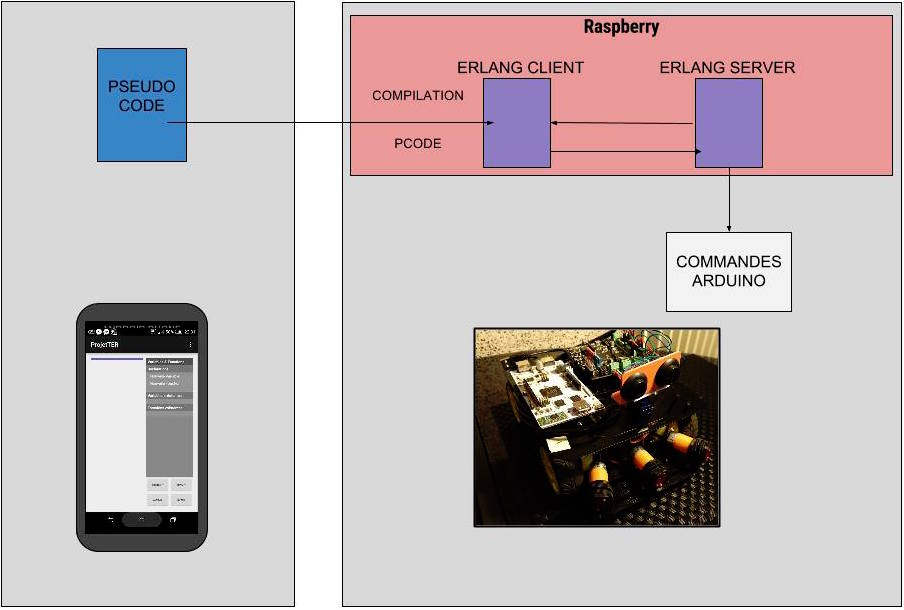
\includegraphics[scale=0.5]{img/archi-erlang.jpg}
\end{center}

Cette méthode profite de la facilité de communication entre plusieurs processus dont dispose Erlang, elle s’avère en premier lieu simple d’implémentations, on pourrait également se demander si une telle architecture ne serait pas simplifiable, et si nos commandes Arduino ne pourraient elles pas découler directement de la compilation.\\
Le PCode nous sers de langage machine, en effet, ce langage proche de l'assembleur nous permettrait de l'interpreter en commande erlang directement éxécutable par le robot.

\vfill\eject
\subsubsection{Pcode}

\begin{center}
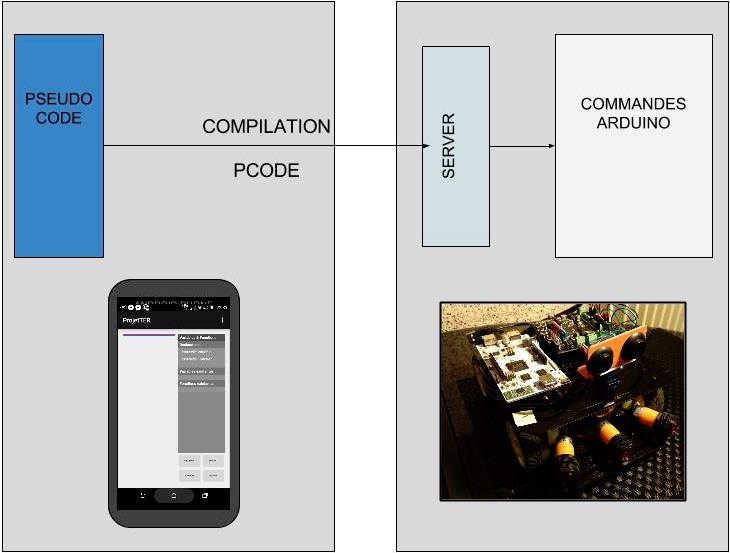
\includegraphics[scale=0.5]{img/archi-pcode.jpg}
\end{center}

Avec cette méthode on allège le cheminement du code, mais on perd le coté pratique de Erlang, c’est une façon plus directe, on passe de notre pseudo code à des commandes Arduino avec plus de transparence. On se sers la encore du PCode comme langage machine intermédiaire, c'est ce PCode qui est interpreté directement par l'Arduino.

\vfill\eject
\subsubsection{Lua}

\begin{center}
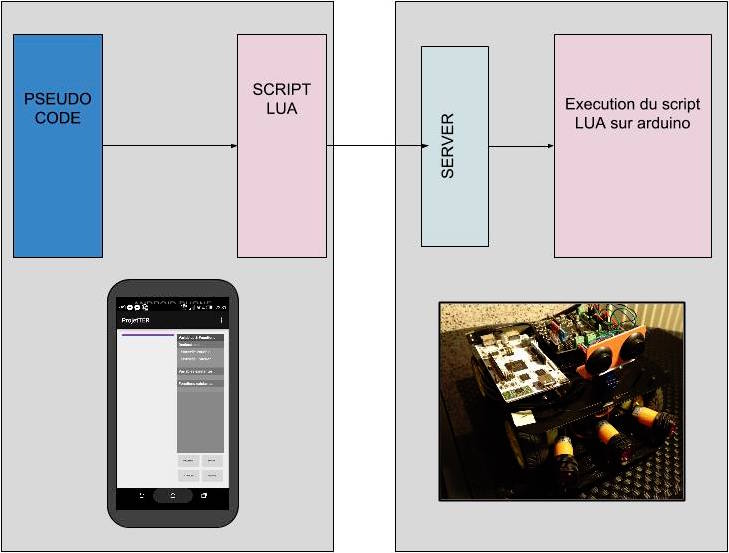
\includegraphics[scale=0.5]{img/archi-lua.jpg}
\end{center}

Cette architecture est basée uniquement sur la capacitée de la carte arduino à recevoir une implementation de LUA Script, si la carte controleur peut éxécuter une version basique de LUA, il est donc possible de directement envoyer un script LUA sur l'arduino, et ce dernier l'éxécutera sans problème sans autre forme de compilation.\\
La seul tâche à effectuer sera de transformer le pseudo code issu de l'interface de l'application android en LUA Script.

\section{Une liste et analyse des besoins fonctionnels}

\subsection{Application}

L’application Android servira à construire un algorithme à travers une interface utilisateur imaginée pour les enfants.

\paragraph{}
L'interface utilisateur de l'application est pensée pour les enfants, il necessite donc de ne pas afficher directement du code face à l'utilisateur, mais plutôt des blocs s'imbriquant les uns les autres pour former un programme. Il est également necessaire d'insister sur les formes et les couleurs afin de rendre l'application ludique pour l'utilisateur. En effet, toutes les combinaisons de blocs possibles qu'offre l'application doivent être éxécutables, afin que l'enfant puisse comprendre directement les conséquences de ses actions, et non se confronter à des erreurs.

\paragraph{}
Les principales inspirations pour l'application fûrent notamment l'application LEGO EV3 et Scratch JR pour tablette, ou les programmes sont composées de blocs tel des pieces d'un puzzle, ou chaque bloc est utilisable independamment et représente une action. Ces deux applications montrent une fenêtre principale dite de "bureau", c'est à dire la fenètre ou l'utilisateur peut faconner librement son programme, en imbriquant les briques les unes avec les autres pour former un algorithme complet.\\
Sous cette fenètre de bureau se trouve un système d'onglet, et chaque onglet correspond à une catégorie de blocs representant une action. Par exemple l'onglet des capteurs proposera des blocs pour lire la valeur de tel ou tel capteurs, l'onglet des actuateurs contiendra des blocs pour actionner les moteurs, jouer un son ou emettre de la lumière.\\

\paragraph{}
Dans l'application LEGO EV3, un onglet flux permet de catégoriser les blocs controlant le déroulement de l'application, on y retrouve donc un bloc "debut" symbolisant le début du programme, ou un bloc "repeter", en forme de C afin de montrer que ce bloc n'est qu'un conteneur pour placer d'autres blocs d'action à l'interieur. Chaque bloc est ainsi personnalisable pour en limiter le nombre de base. Par exemple le bloc "jouer un son", une fois placé dans le programme, va permettre de choisir quel type de son jouer, et à quelle intensitée pendant combien de temps.

\paragraph{}
Dans l'application Scratch JR, étant plus adaptée aux enfants, on remarque la possibilitée d'importer et de modifier ses propres images et son depuis la tablette, afin d'offrir des capacités de personnalisation poussée du programme, pour que l'enfant s'identifie plus au projet. Il est également necessaire que l'espace de travail sois perçu comme un bureau physique, ou l'on peut laisser des blocs de côté, afin d'être réutilisé plus tard, ou seul les blocs colés après le bloc "debut" sont pris en compte dans l'éxécution finale

\subsection{Robot}

\begin{center}
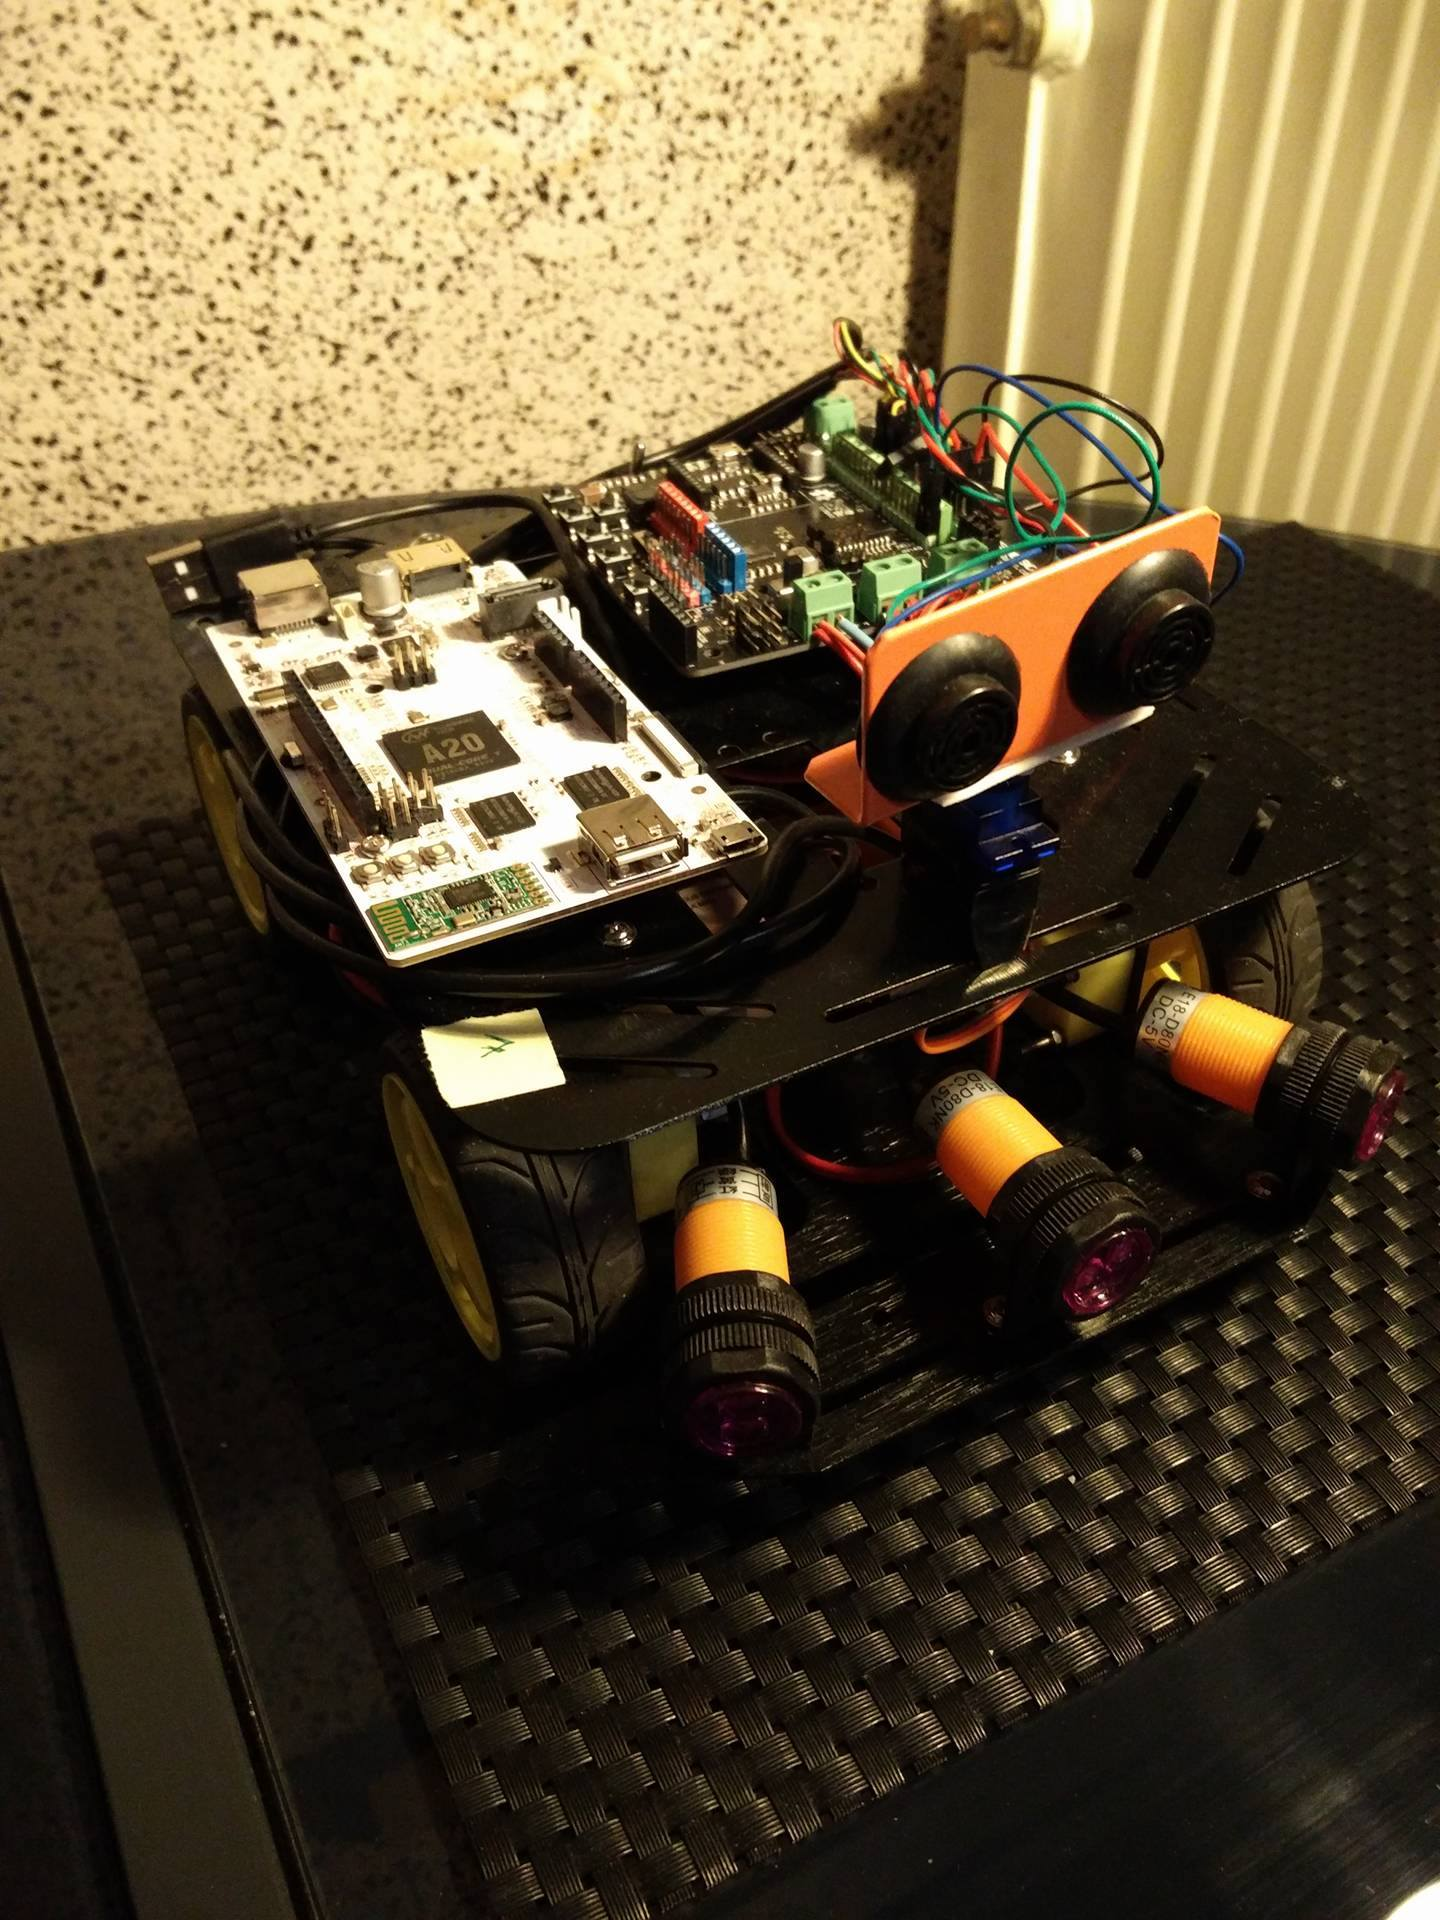
\includegraphics[scale=0.15]{img/robot.jpg}
\end{center}

\paragraph{}
Le robot est, dans le cadre du projet, composé :
\begin{itemize}
\item D'un chassis à 4 roues motrices, sur lequel viens se fixer les differents capteurs, moteurs et carte élétroniques
\item De 4 roues motrices actionnés par une batterie externe pour délivrer plus de puissance
\item D'un capteur à ultrasons, posté sur un servo-moteur
\item De 3 capteurs de proximités infrarouges
\item D'une carte controleur de type Romeo, basée sur un Arduino Leonardo
\item D'un mini pc tel un raspberry pi, avec wifi et bluetooth, fonctionnant sous ubuntu qui est relié en USB à la carte contrôleur
\item De deux batterie, une pour la carte contrôleur et le mini pc, l'autre spécifique pour les moteurs
\end{itemize}

\paragraph{}
Le but du robot est de communiquer en direct avec l'application Android via Wifi, afin de recevoir le code produit par l'utilisateur sur l'application, et selon l'architecture choisis de directement l'éxécuter sur l'arduino, ou de préalablement recompiler ce code pour l'éxécuter ensuite.\\
Il sera par la suite possible d'améliorer ce robot afin d'ajout differents capteurs, ou même de se passer du mini pc si les instructions passée à l'arduino sont déjà pré-compilées par le téléphone afin de les envoyer directement à la carte contrôleur via un shield Arduino Wifi, cela baisserait drastiquement la taille et le coup de production du dit robot.

\subsection{Mini-Langage}

Le développement d’un mini-langage est crucial dans ce projet, en effet, l’application ne sers que d’interface pour facilement écrire ce langage, qui sera traduit de manière formelle via l’application. Ce langage formel, défini via une grammaire, subira plusieurs phases d’analyse soit : lexicale, syntaxique et sémantique, afin de traduire ce mini-langage dans un langage machine exécutable sur le robot afin d’effectuer les requêtes de l’utilisateur.

\paragraph{}
Ce mini-langage sera une interpretation du "bureau" de l'application, c'est à dire de la suite de blocs prise en compte dans le programme final. Le langage cible sera donc une serie de commande très simple, envoyée sur le port serie de l'Arduino ou directement via wifi si une architecture sans mini pc est choisie, afin que ces commandes sois directement comprise et éxécutées via le code de la carte controlleur arduino.

\section{Une description de prototypes et des résultats de tests préparatoires}
\subsection{Prototype android}
\begin{center}
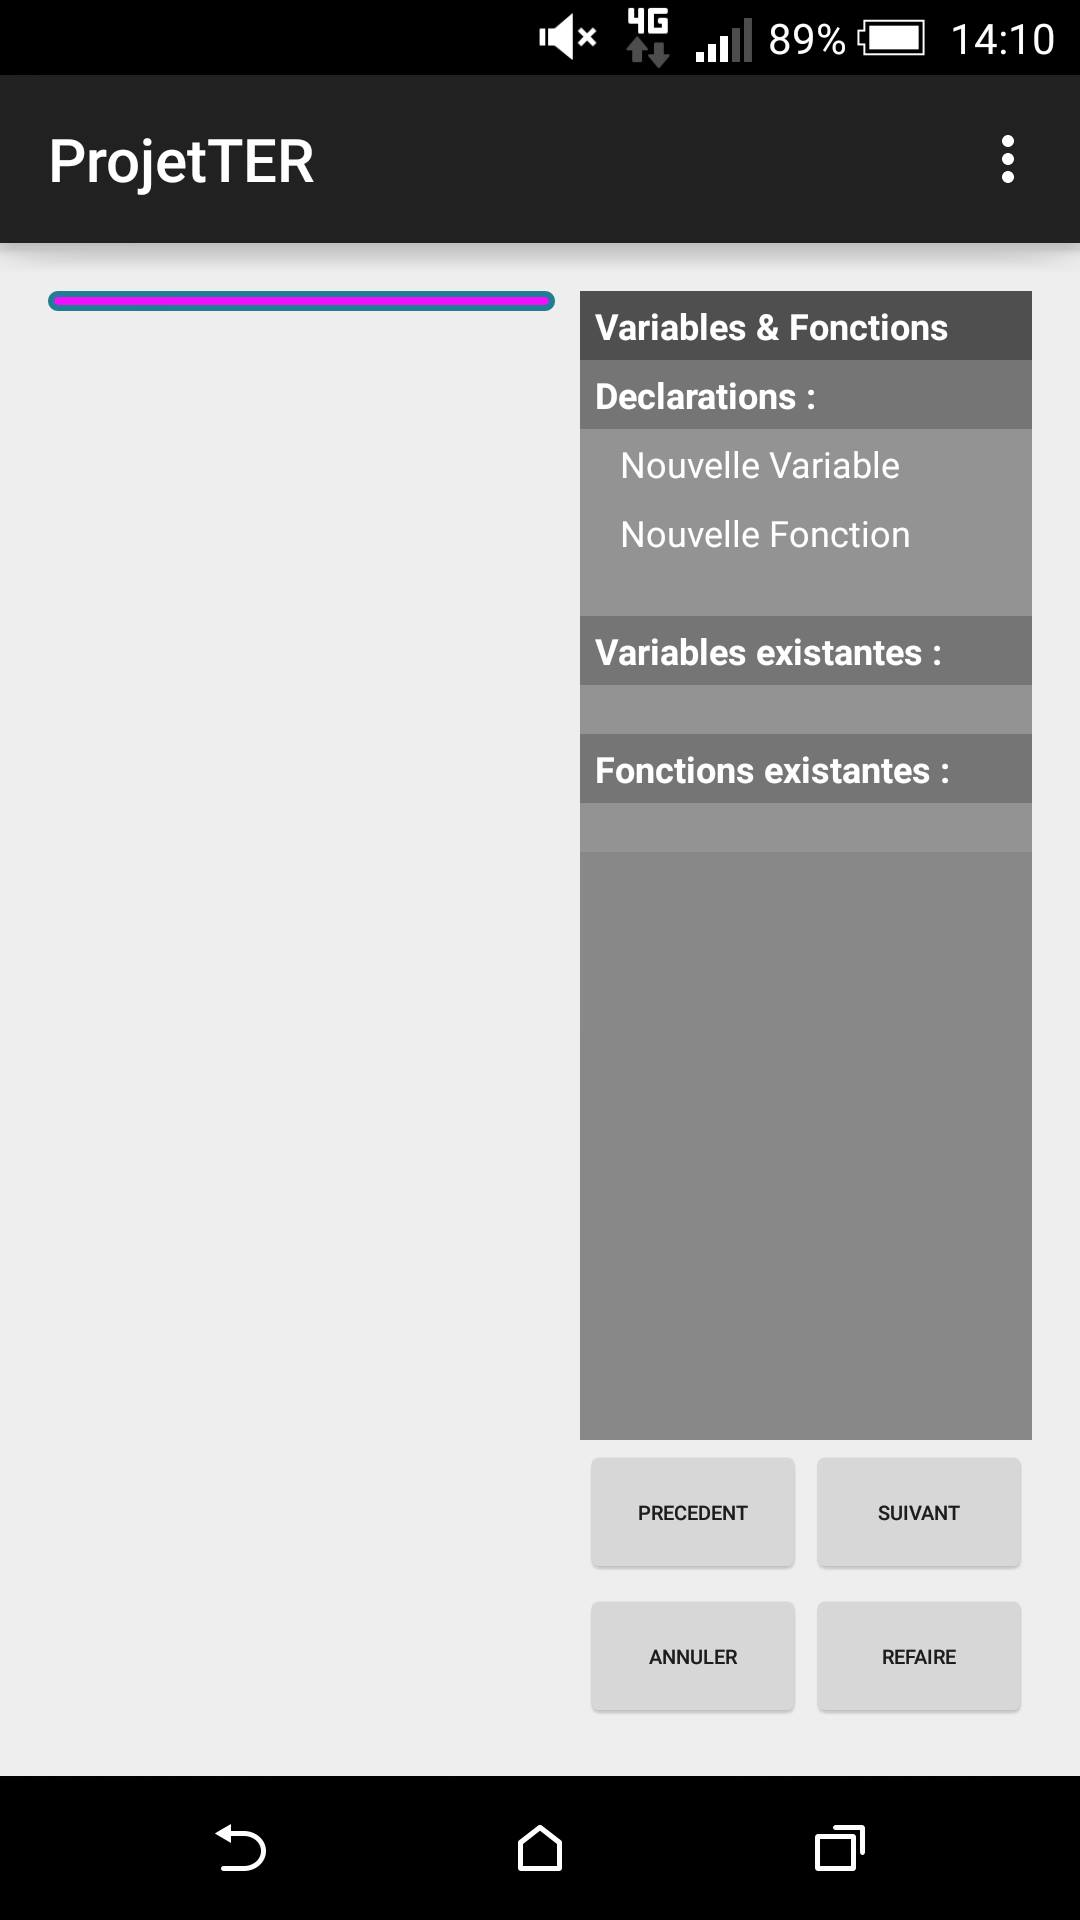
\includegraphics[scale=0.1]{img/menu_variableFonctions.jpg}
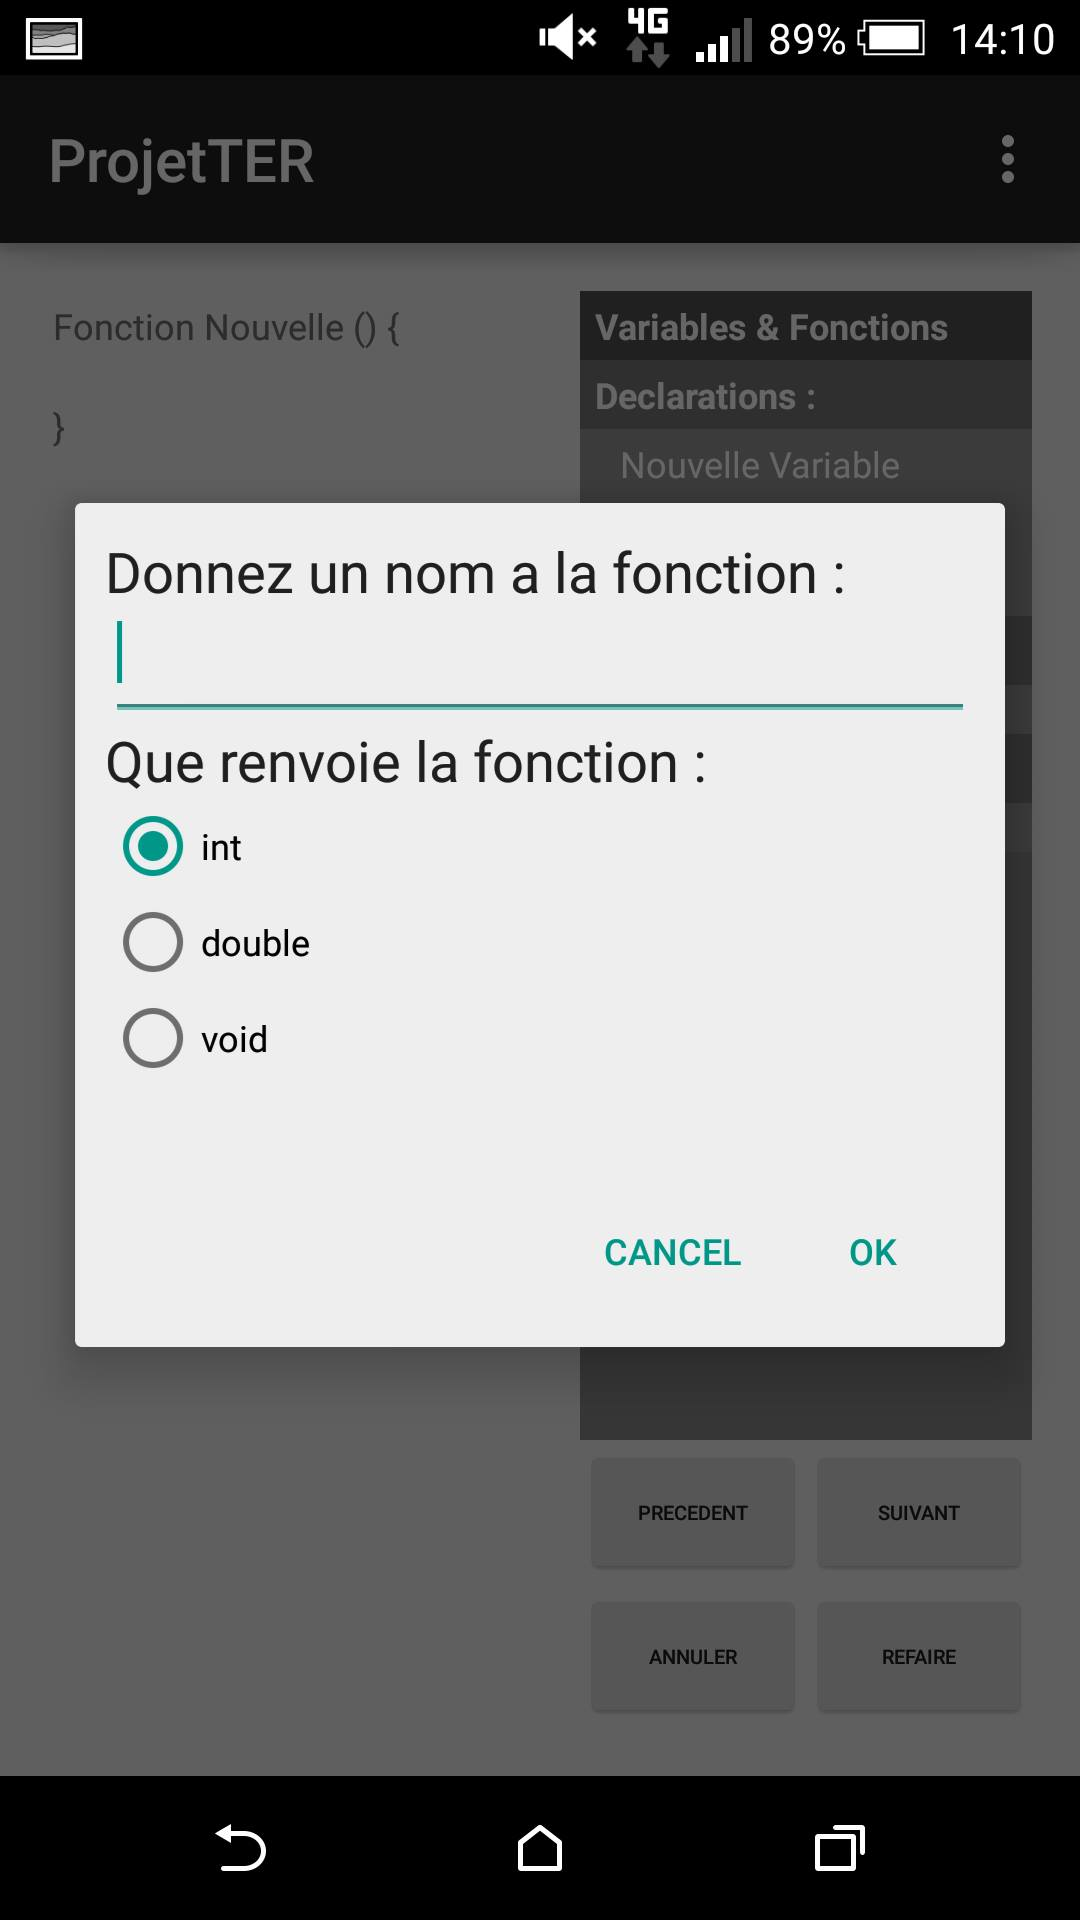
\includegraphics[scale=0.1]{img/popup_fonction.jpg}
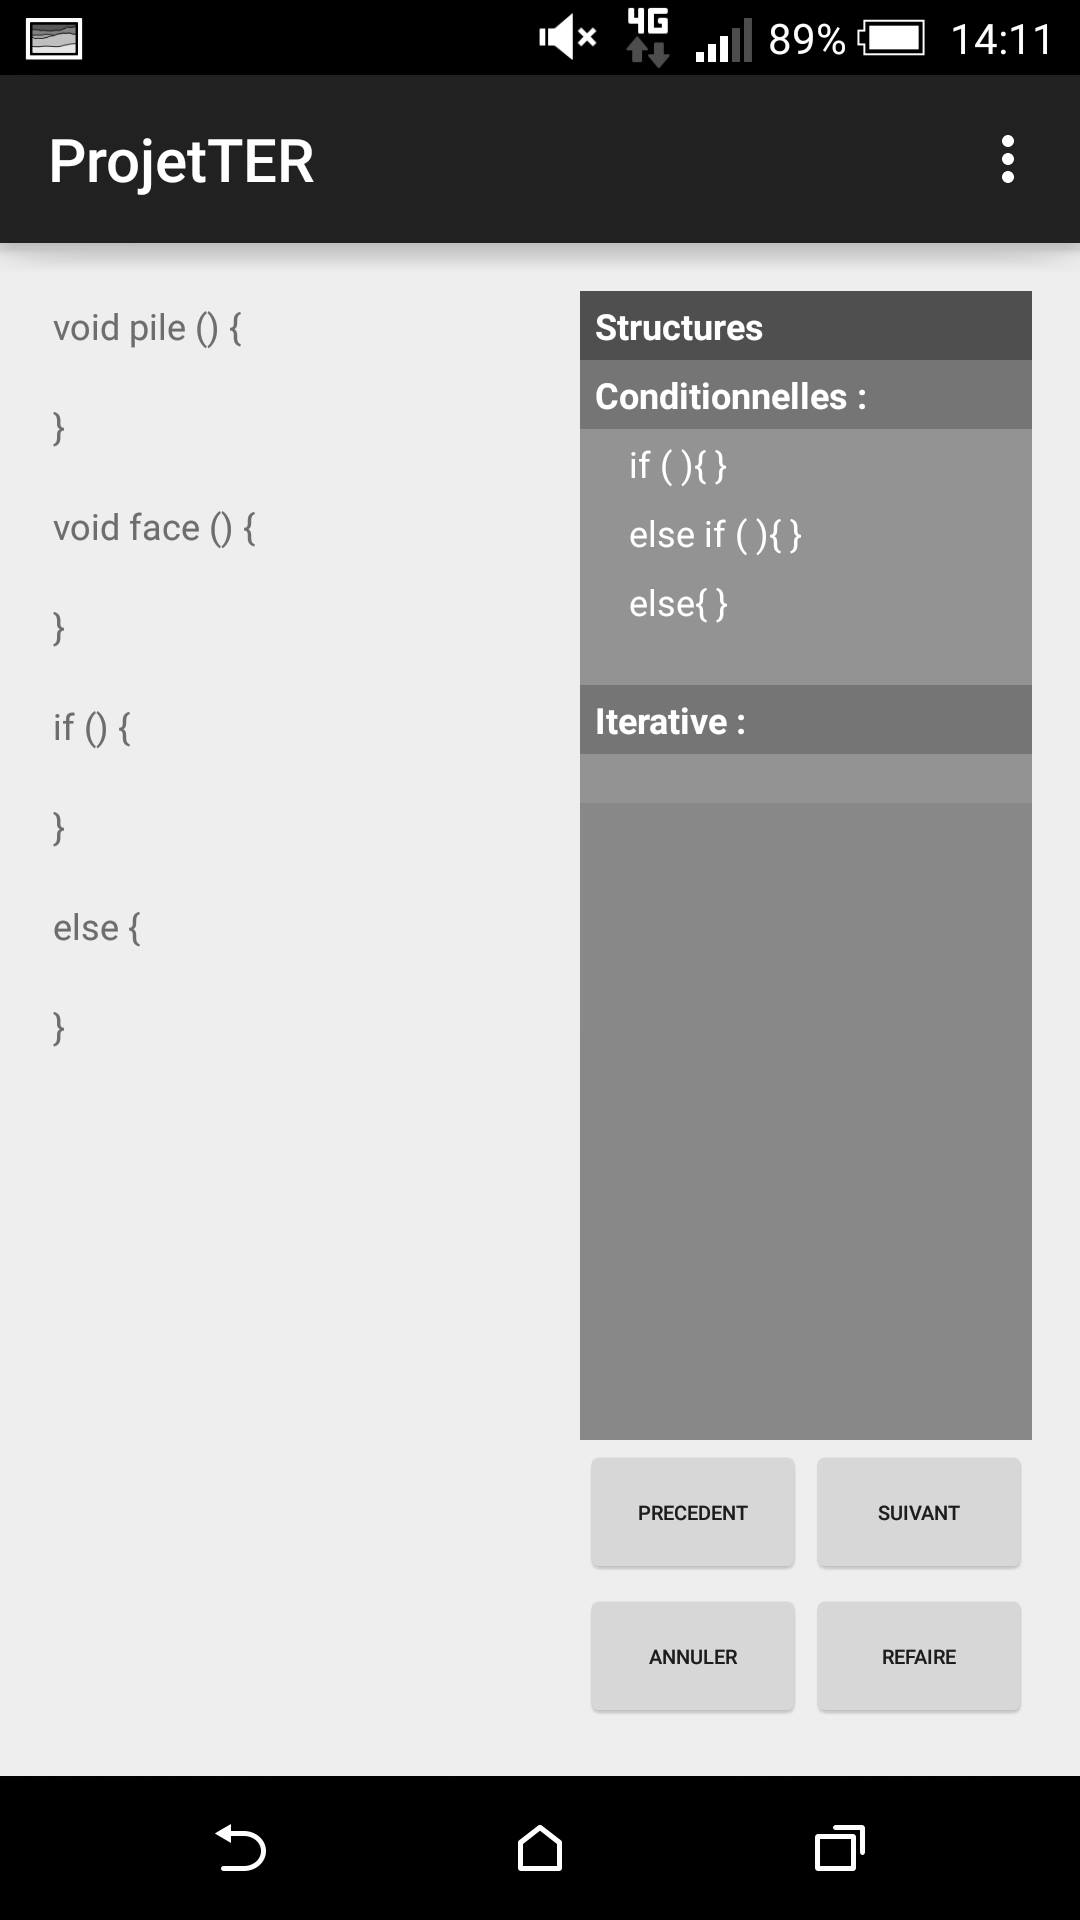
\includegraphics[scale=0.1]{img/create1.jpg}
\end{center}
Une Viewanimator à droite, contenant liste de scrollview contenant différents élément de programmations tel que les structures (conditionnelles et boucles), les variables ou encore les opérateur de calculs et logique. Les différents éléments peuvent être drag and drop vers d’autres vues. \\
\\
\begin{center}
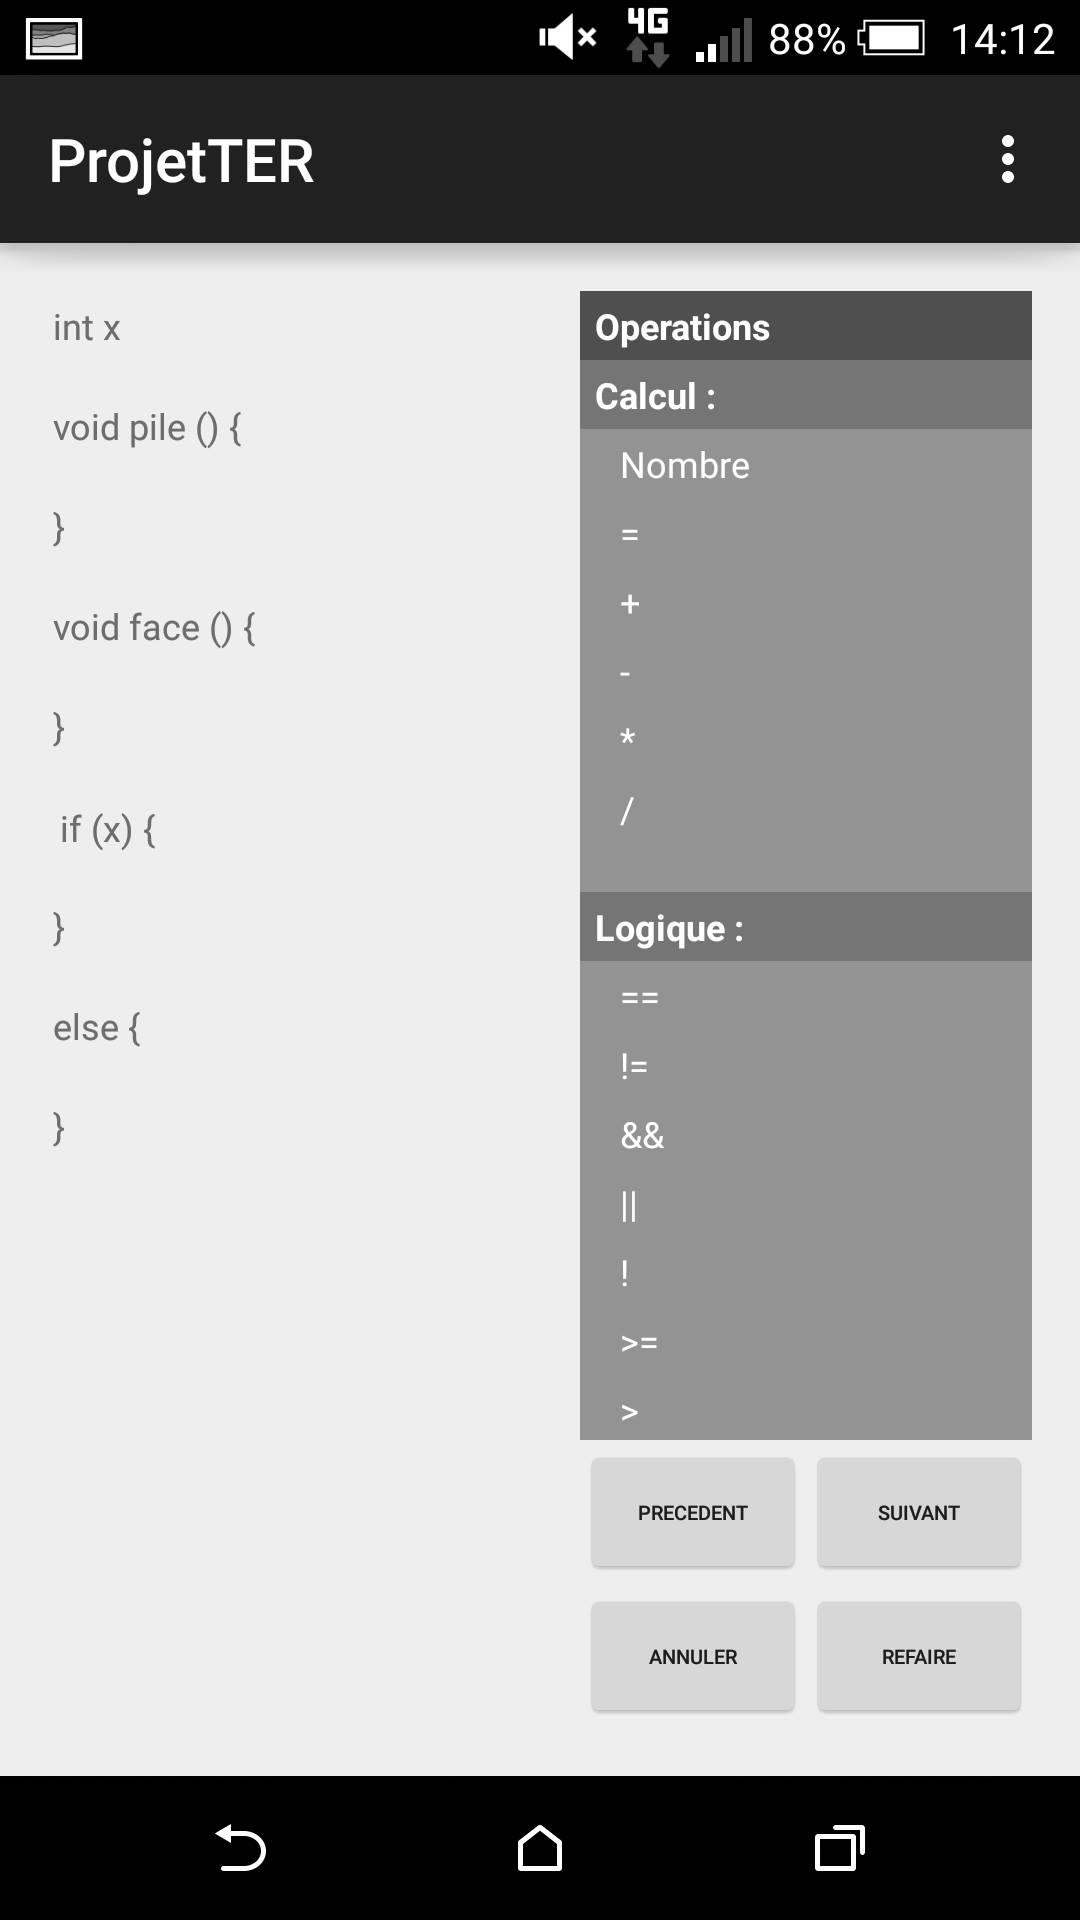
\includegraphics[scale=0.1]{img/create2.jpg}
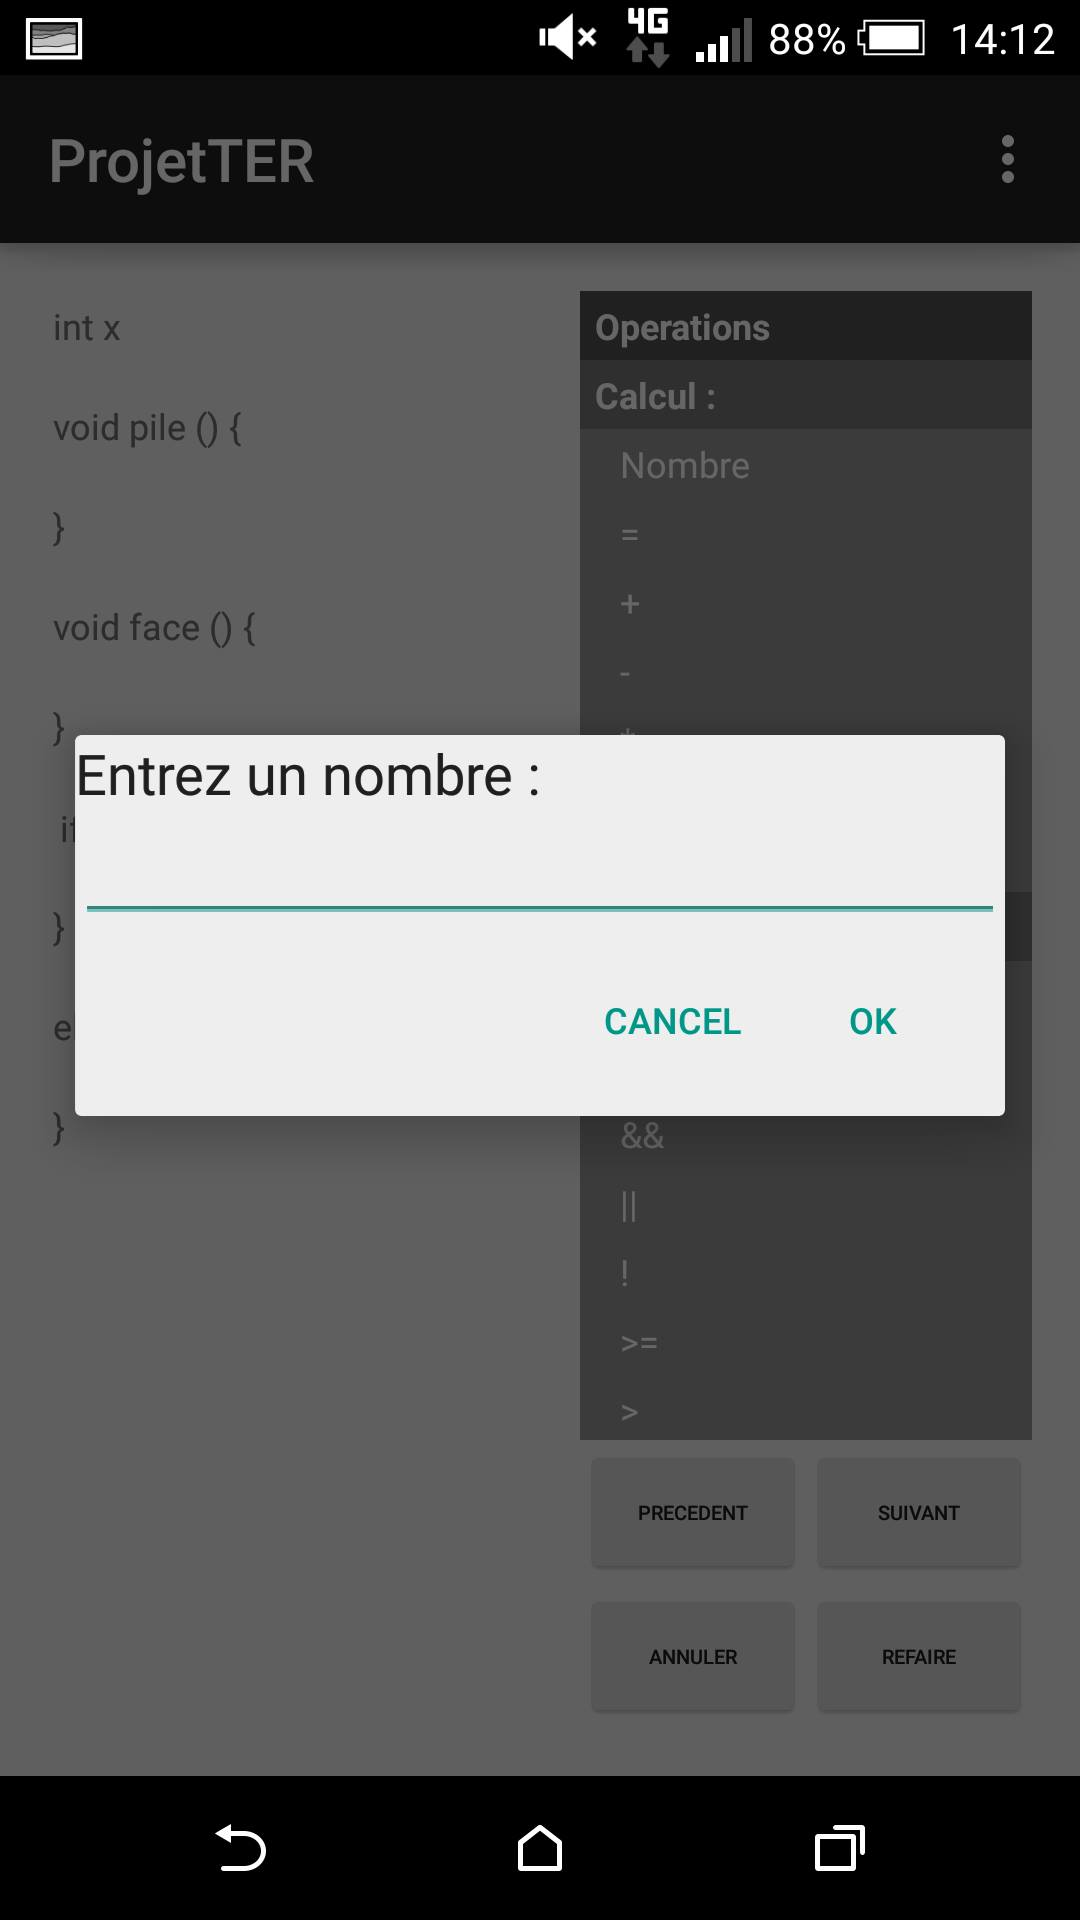
\includegraphics[scale=0.1]{img/popup_nombre.jpg}
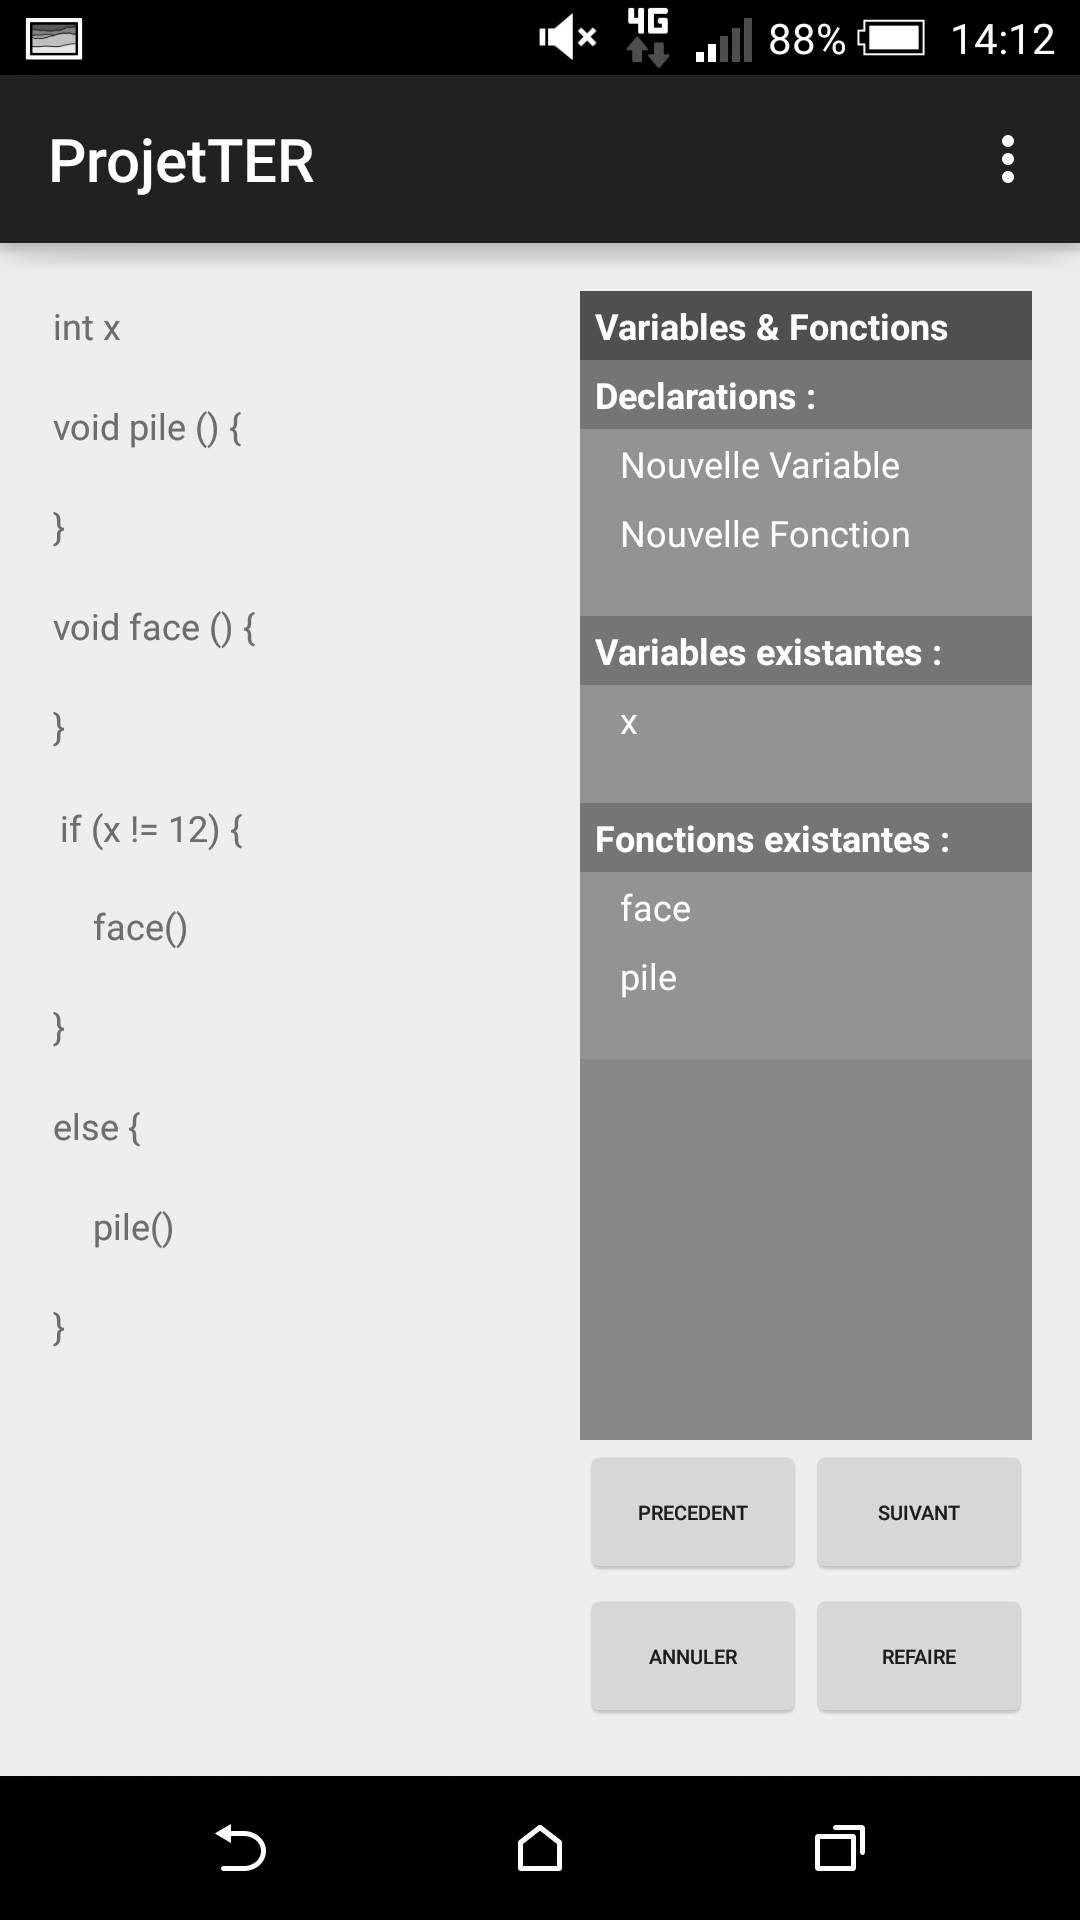
\includegraphics[scale=0.1]{img/create3.jpg}
\end{center}

Scrollview a gauche servant de réceptacle aux éléments de codes. Lors du drag and drop, soit les élément donnent lieu a une nouvelle ligne de code, soit les élément enrichissent les lignes deja présentes (exemple : drop d’une variable dans un if)

\subsection{Prototype robot}

Un code arduino à été écris afin de comprendre des instructions basiques envoyées sur son port serie, et exécute des insctructions en fonctions de la commande reçue.\\
Par exemple, on peut envoyer la suite de commande "w w w a s d" sur le port serie, qui aura pour effet de faire avancer 3 fois pendant 1 secondes le robot vers l'avant, puis de le faire tourner à gauche pendant une seconde, le faire reculer puis tourner à droite pendant une seconde.\\

\paragraph{}
Pour éviter tout dommage sur le robot, des routines dites "de sécurité" sont mises en place dans le code de l'arduino, ces routines permettent d'éviter au robot d'entrer en collision avec tout obstacle présent sur sa route. En effet, le robot verifie en permanence l'espace devant lui, et va chercher à tout prix à éviter la collision avec un obstacle, et cela même si l'instruction du programme qu'il est en train d'éxécuter lui indique d'aller vers cette collision.\\
Cette vérification pourra être désactivée mais sera déconseillée, car un choc à pleine vitesse peut avoir de graves conséquences sur l'intégrité du robot.

\subsection{Prototype compilateur}
Définition d’une grammaire via un outil d’analyse lexicale et sémantique, ATNLR4, qui permet via la description d’expressions régulières combinée de formuler un langage.\\
\\
Une fois cette grammaire définie, l’outil permet de créer un AST, qui permet ensuite d’effectuer l’analyse sémantique via une table des symboles, ce qui aboutira à la production du code machine exécutable sur le robot
\section{Un planning, affectations des tâches}

Victor : mini-langage et compilateur\\
Julien et Vladimir: travail sur l’application\\

\vfill\eject
\bibliographystyle{plain}
\bibliography{rapport}
\end{document}
